\documentclass[tikz,border=2pt]{standalone}
\usepackage[T1]{fontenc}
\usepackage[utf8]{inputenc}
\usepackage{amsmath,amssymb}

% ACM
%\usepackage[tt=false, type1=true]{libertine}
%\usepackage[varqu]{zi4}
%\usepackage[libertine]{newtxmath}

% IEEE
\renewcommand{\sfdefault}{phv}
\renewcommand{\rmdefault}{ppl}
\renewcommand{\ttdefault}{pcr}
\usepackage{mathptmx}

\usepackage{pgfplots}
\pgfplotsset{compat=1.18}
\usepgfplotslibrary{groupplots}
\usepgfplotslibrary{colormaps}
\tikzset{
	fill-color/.style={
		color of colormap={#1},
		draw=.!80!black,
		fill=.!80!white,
	},
	normal-color/.style={
		color of colormap={#1},
		draw=.,
	},
	mydashed/.style={dash pattern=on 6pt off 4pt}
}

\makeatletter
\pgfplotsset{
	groupplot xlabel/.initial={},
	every groupplot x label/.style={
		at={($({\pgfplots@group@name\space c1r\pgfplots@group@rows.west}|-{\pgfplots@group@name\space c1r\pgfplots@group@rows.outer south})!0.5!({\pgfplots@group@name\space c\pgfplots@group@columns r\pgfplots@group@rows.east}|-{\pgfplots@group@name\space c\pgfplots@group@columns r\pgfplots@group@rows.outer south})$)},
		yshift=2ex,
		anchor=north,
	},
	groupplot ylabel/.initial={},
	every groupplot y label/.style={
		rotate=90,
		at={($({\pgfplots@group@name\space c1r1.north}-|{\pgfplots@group@name\space c1r1.outer
				west})!0.5!({\pgfplots@group@name\space c1r\pgfplots@group@rows.south}-|{\pgfplots@group@name\space c1r\pgfplots@group@rows.outer west})$)},
		anchor=south
	},
	execute at end groupplot/.code={%
		\node [/pgfplots/every groupplot x label]
		{\pgfkeysvalueof{/pgfplots/groupplot xlabel}};  
		\node [/pgfplots/every groupplot y label] 
		{\pgfkeysvalueof{/pgfplots/groupplot ylabel}};  
	}
}

\def\endpgfplots@environment@groupplot{%
	\endpgfplots@environment@opt%
	\pgfkeys{/pgfplots/execute at end groupplot}%
	\endgroup%
}
\makeatother

% Code from Christian Feuersänger
% https://tex.stackexchange.com/questions/54794/using-a-pgfplots-style-legend-in-a-plain-old-tikzpicture#54834

% argument #1: any options
\newenvironment{customlegend}[1][]{%
	\begingroup
	% inits/clears the lists (which might be populated from previous
	% axes):
	\csname pgfplots@init@cleared@structures\endcsname
	\pgfplotsset{#1}%
}{%
	% draws the legend:
	\csname pgfplots@createlegend\endcsname
	\endgroup
}%

% makes \addlegendimage available (typically only available within an
% axis environment):
\def\addlegendimage{\csname pgfplots@addlegendimage\endcsname}


\begin{document}
% This file was created with tikzplotlib v0.10.1.
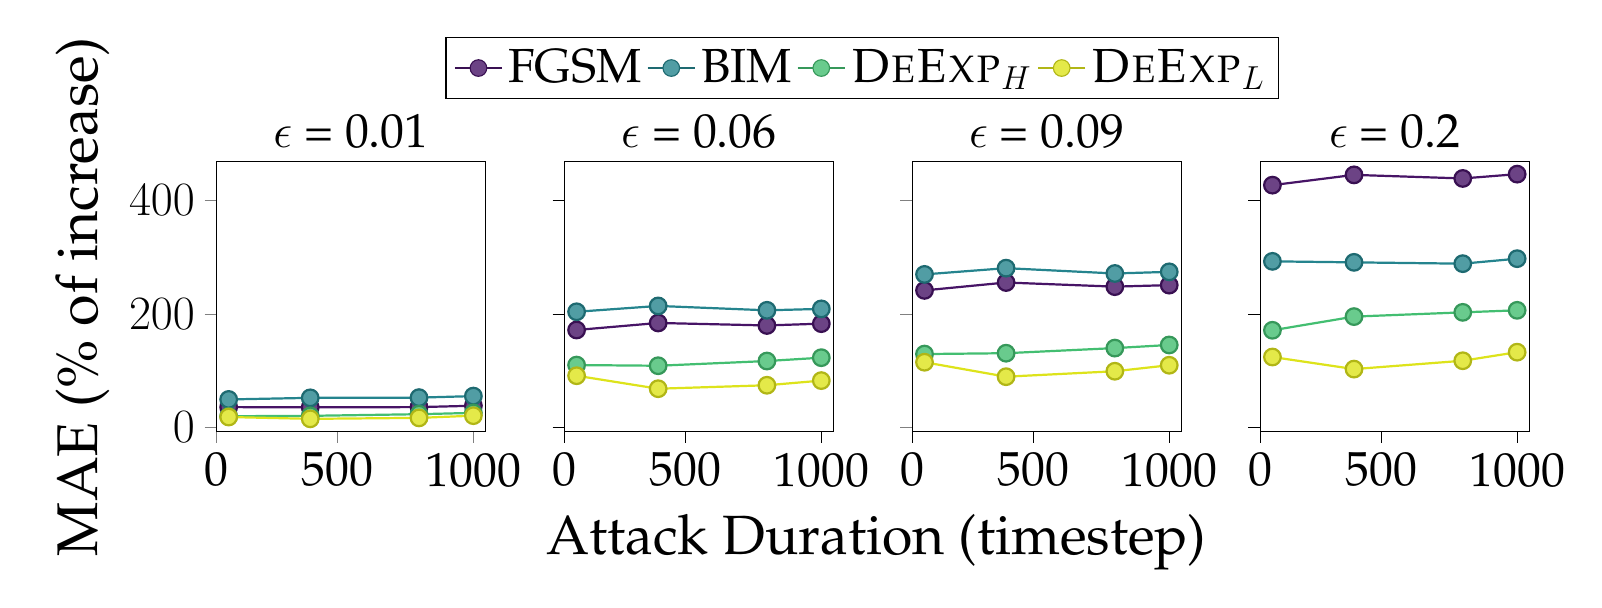
\begin{tikzpicture}

\definecolor{darkgray176}{RGB}{176,176,176}
\definecolor{green}{RGB}{0,128,0}
\definecolor{lightgray204}{RGB}{204,204,204}
\definecolor{purple}{RGB}{128,0,128}
\definecolor{yellow}{RGB}{255,255,0}

\begin{groupplot}[group style={group size=4 by 1},
width=5cm, height = 5cm,
xlabel style={font=\huge},
ylabel style={font=\huge},
xticklabel style={font=\LARGE},
yticklabel style={font=\LARGE},
title style={font=\LARGE,yshift=-1ex},
groupplot xlabel = {\fontsize{20}{33} \selectfont Attack Duration (timestep)},
xtick={55,500,1000},
xticklabels={0,500,1000},
yticklabel style={%
	scaled y ticks = false,
	/pgf/number format/.cd,
	fixed,
	precision=0,
	fixed zerofill,
	1000 sep={\,},
},
xticklabel style={%
	scaled y ticks = false,
	/pgf/number format/.cd,
	fixed,
	precision=0,
	fixed zerofill,
	1000 sep={\,},
},colormap/viridis
]
\nextgroupplot[
tick align=outside,
tick pos=left,
title={\(\displaystyle \epsilon\) = 0.01},
xmin=55, xmax=1045,
ylabel={MAE (\% of increase)},
ymin=-6.465, ymax=467.965,
colormap/viridis,
]
% (Relative) Coordinate at top of the first plot
\coordinate (c1) at (rel axis cs:0,1);% I moved this to the upper left corner

\addplot [thick, normal-color={50}, mark=*, mark size=3, mark options={solid,fill-color={50}}]
table {%
100 35.8
400 35.4
800 35.8
1000 38.2
};
\addplot [thick, normal-color={450}, mark=*, mark size=3, mark options={solid,fill-color={450}}]
table {%
100 49.3
400 52.1
800 52.5
1000 55.2
};
\addplot [thick, normal-color={700}, mark=*, mark size=3, mark options={solid,fill-color={700}}]
table {%
100 19.7
400 20.4
800 23.3
1000 25.6
};
\addplot [thick, normal-color={950}, mark=*, mark size=3, mark options={solid,fill-color={950}}]
table {%
100 18.3
400 15.1
800 16.8
1000 20.7
};

\nextgroupplot[
scaled y ticks=manual:{}{\pgfmathparse{#1}},
tick align=outside,
tick pos=left,
title={\(\displaystyle \epsilon\) = 0.06},
x grid style={darkgray176},
xmin=55, xmax=1045,
xtick style={color=black},
y grid style={darkgray176},
ymin=-6.465, ymax=467.965,
ytick style={color=black},
yticklabels={}
]
\addplot [thick, normal-color={50}, mark=*, mark size=3, mark options={solid,fill-color={50}}]
table {%
100 171.7
400 184.1
800 179.7
1000 182.9
};
\addplot [thick, normal-color={450}, mark=*, mark size=3, mark options={solid,fill-color={450}}]
table {%
100 203.8
400 214.1
800 206.4
1000 208.9
};
\addplot [thick, normal-color={700}, mark=*, mark size=3, mark options={solid,fill-color={700}}]
table {%
100 109.9
400 108.7
800 117
1000 122.9
};
\addplot [thick, normal-color={950}, mark=*, mark size=3, mark options={solid,fill-color={950}}]
table {%
100 91.1
400 68.2
800 74.3
1000 82.5
};

\nextgroupplot[
scaled y ticks=manual:{}{\pgfmathparse{#1}},
tick align=outside,
tick pos=left,
title={\(\displaystyle \epsilon\) = 0.09},
xmin=55, xmax=1045,
xtick style={color=black},
ymin=-6.465, ymax=467.965,
yticklabels={}
]
\addplot [thick, normal-color={50}, mark=*, mark size=3, mark options={solid,fill-color={50}}]
table {%
100 241.5
400 255.4
800 248.1
1000 250.8
};
\addplot [thick, normal-color={450}, mark=*, mark size=3, mark options={solid,fill-color={450}}]
table {%
100 269.7
400 280.7
800 271.3
1000 274.2
};
\addplot [thick, normal-color={700}, mark=*, mark size=3, mark options={solid,fill-color={700}}]
table {%
100 129.3
400 130.8
800 139.8
1000 145.3
};
\addplot [thick, normal-color={950}, mark=*, mark size=3, mark options={solid,fill-color={950}}]
table {%
100 114.9
400 89.4
800 99
1000 109.6
};

\nextgroupplot[
scaled y ticks=manual:{}{\pgfmathparse{#1}},
tick align=outside,
tick pos=left,
title={\(\displaystyle \epsilon\) = 0.2},
x grid style={darkgray176},
xmin=55, xmax=1045,
xtick style={color=black},
y grid style={darkgray176},
ymin=-6.465, ymax=467.965,
ytick style={color=black},
yticklabels={}
]
\addplot [thick, normal-color={50}, mark=*, mark size=3, mark options={solid,fill-color={50}}]
table {%
100 427
400 445.1
800 438.8
1000 446.4
};
\addplot [thick, normal-color={450}, mark=*, mark size=3, mark options={solid,fill-color={450}}]
table {%
100 292.7
400 290.9
800 288.6
1000 297.4
};
\addplot [thick, normal-color={700}, mark=*, mark size=3, mark options={solid,fill-color={700}}]
table {%
100 171.2
400 195.3
800 202.8
1000 206.4
};
\addplot [thick, normal-color={950}, mark=*, mark size=3, mark options={solid,fill-color={950}}]
table {%
100 124.1
400 102.8
800 117.5
1000 132.6
};
\end{groupplot}
\begin{customlegend}[colormap/viridis,
	legend entries={ % <= in the following there are the entries
		FGSM,
		BIM,
		\textsc{DeExp}$_H$,
		\textsc{DeExp}$_L$,
	},
	legend columns=-1,
	legend style={at={(13.5,5)},font=\LARGE}] % <= to define position and font legend
	% the following are the "images" and numbers in the legend
	\addlegendimage{fill-color={50}, mark=*, mark size=3, mark options={solid}}
	\addlegendimage{fill-color={450}, mark=*, mark size=3, mark options={solid}}
	\addlegendimage{fill-color={700}, mark=*, mark size=3, mark options={solid}}
	\addlegendimage{fill-color={950}, mark=*, mark size=3, mark options={solid}}
\end{customlegend}
\end{tikzpicture}
\end{document}